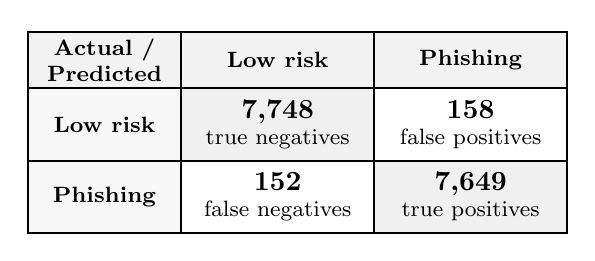
\begin{tikzpicture}[
  font=\footnotesize,
  header/.style={font=\footnotesize\bfseries, align=center},
  label/.style={font=\footnotesize\bfseries, align=center},
  value/.style={align=center},
]
\def\wlabel{1.95}
\def\wcell{2.45}
\def\hhead{0.72}
\def\hcell{0.92}
\def\xone{\wlabel}
\def\xtwo{4.40}
\def\xthree{6.85}
\def\yone{-\hhead}
\def\ytwo{-1.64}
\def\ythree{-2.56}

\path[use as bounding box] (0.0,0.05) rectangle (\xthree,\ythree);

\fill[gray!10] (0,0) rectangle (\xone,\yone);
\fill[gray!10] (\xone,0) rectangle (\xtwo,\yone);
\fill[gray!10] (\xtwo,0) rectangle (\xthree,\yone);
\fill[gray!6] (0,\yone) rectangle (\xone,\ytwo);
\fill[gray!6] (0,\ytwo) rectangle (\xone,\ythree);
\fill[gray!12] (\xone,\yone) rectangle (\xtwo,\ytwo);
\fill[gray!12] (\xtwo,\ytwo) rectangle (\xthree,\ythree);

\draw[thick] (0,0) rectangle (\xthree,\ythree);
\draw[thick] (\xone,0) -- (\xone,\ythree);
\draw[thick] (\xtwo,0) -- (\xtwo,\ythree);
\draw[thick] (0,\yone) -- (\xthree,\yone);
\draw[thick] (0,\ytwo) -- (\xthree,\ytwo);

\node[header] at (0.975,-0.36) {Actual /\\Predicted};
\node[header] at (3.175,-0.36) {Low risk};
\node[header] at (5.625,-0.36) {Phishing};

\node[label] at (0.975,-1.18) {Low risk};
\node[label] at (0.975,-2.10) {Phishing};

\node[value] at (3.175,-1.18) {{\normalsize\bfseries 7,748}\\true negatives};
\node[value] at (5.625,-1.18) {{\normalsize\bfseries 158}\\false positives};
\node[value] at (3.175,-2.10) {{\normalsize\bfseries 152}\\false negatives};
\node[value] at (5.625,-2.10) {{\normalsize\bfseries 7,649}\\true positives};
\end{tikzpicture}
